\documentclass[14pt,a4paper]{extarticle}

\usepackage{fontspec}
\setmainfont{Times New Roman}
\setsansfont{Helvetica}
\usepackage{polyglossia}
\setdefaultlanguage{russian}
\setotherlanguage{english}
\newfontfamily\russianfonttt{Courier New}

\usepackage[left=30mm,right=15mm,top=20mm,bottom=20mm]{geometry}
\usepackage{setspace}
\onehalfspacing
\usepackage{indentfirst}
\setlength{\parindent}{1.25cm}

\tolerance=9000
\emergencystretch=3em
\hbadness=10000
\setlength{\overfullrule}{0pt}

\usepackage{graphicx}
\usepackage{float}

\usepackage{caption}
\captionsetup[figure]{name=Рисунок,labelsep=endash}

\usepackage{fancyhdr}
\pagestyle{fancy}
\fancyhf{}
\fancyfoot[C]{\thepage}
\renewcommand{\headrulewidth}{0pt}

\usepackage[hidelinks]{hyperref}

\usepackage{listings}
\lstset{
  basicstyle=\small\ttfamily,
  breaklines=true,
  frame=single,
  xleftmargin=1.25cm,
  numbers=left,
  numberstyle=\tiny,
  showstringspaces=false,
  tabsize=4,
}

\begin{document}

\thispagestyle{empty}
\begin{center}
\textbf{МИНИСТЕРСТВО НАУКИ И ВЫСШЕГО ОБРАЗОВАНИЯ РОССИЙСКОЙ ФЕДЕРАЦИИ}\\[0.3cm]
\textbf{УНИВЕРСИТЕТ ИТМО}\\[0.5cm]
Факультет ПИиКТ\\[1.5cm]

\textbf{\Large Лабораторная работа №3}\\[0.5cm]
\textbf{\large ASP.NET MVC}\\[0.5cm]
по дисциплине <<Создание программного обеспечения>>\\[2cm]
\end{center}

\begin{flushleft}
\hspace{1.25cm}\begin{minipage}[t]{\dimexpr\textwidth-1.25cm\relax}
\textbf{Выполнил:} студент Луценко Владимир\\
\textbf{Группа:} К3420\\
\textbf{Преподаватель:} Осипов Н. А.\\
\end{minipage}
\end{flushleft}

\vfill
\begin{center}
Санкт-Петербург, 2026
\end{center}
\newpage

\tableofcontents
\newpage

\section{Введение}

Цель работы -- освоение технологии ASP.NET Core MVC. В рамках лабораторных работ 5--8 разработано приложение MvcCreditApp для управления кредитными продуктами: создана модель данных, реализованы CRUD-контроллеры, добавлен AJAX-поиск и настроена авторизация через Identity.

\section{ЛР 5. Разработка модели}

Создан проект ASP.NET Core MVC с шаблоном Individual User Accounts и базой данных SQLite. Определены модели \texttt{Credit} (кредитный продукт) и \texttt{Bid} (заявка). Контекст \texttt{CreditContext} содержит \texttt{DbSet} для обеих сущностей.

\begin{lstlisting}[caption={Модель Credit.cs},language={[Sharp]C}]
public class Credit
{
    public int CreditId { get; set; }
    [DisplayName("Название")]
    [Required]
    public string Head { get; set; }
    [DisplayName("Срок (мес.)")]
    public int Period { get; set; }
    [DisplayName("Сумма")]
    public decimal Sum { get; set; }
    [DisplayName("Процент")]
    public double Procent { get; set; }
}
\end{lstlisting}

Класс \texttt{SeedData} добавляет 5 тестовых кредитов при первом запуске. В \texttt{HomeController} выводится таблица кредитов и форма подачи заявки.

\begin{figure}[H]
\centering
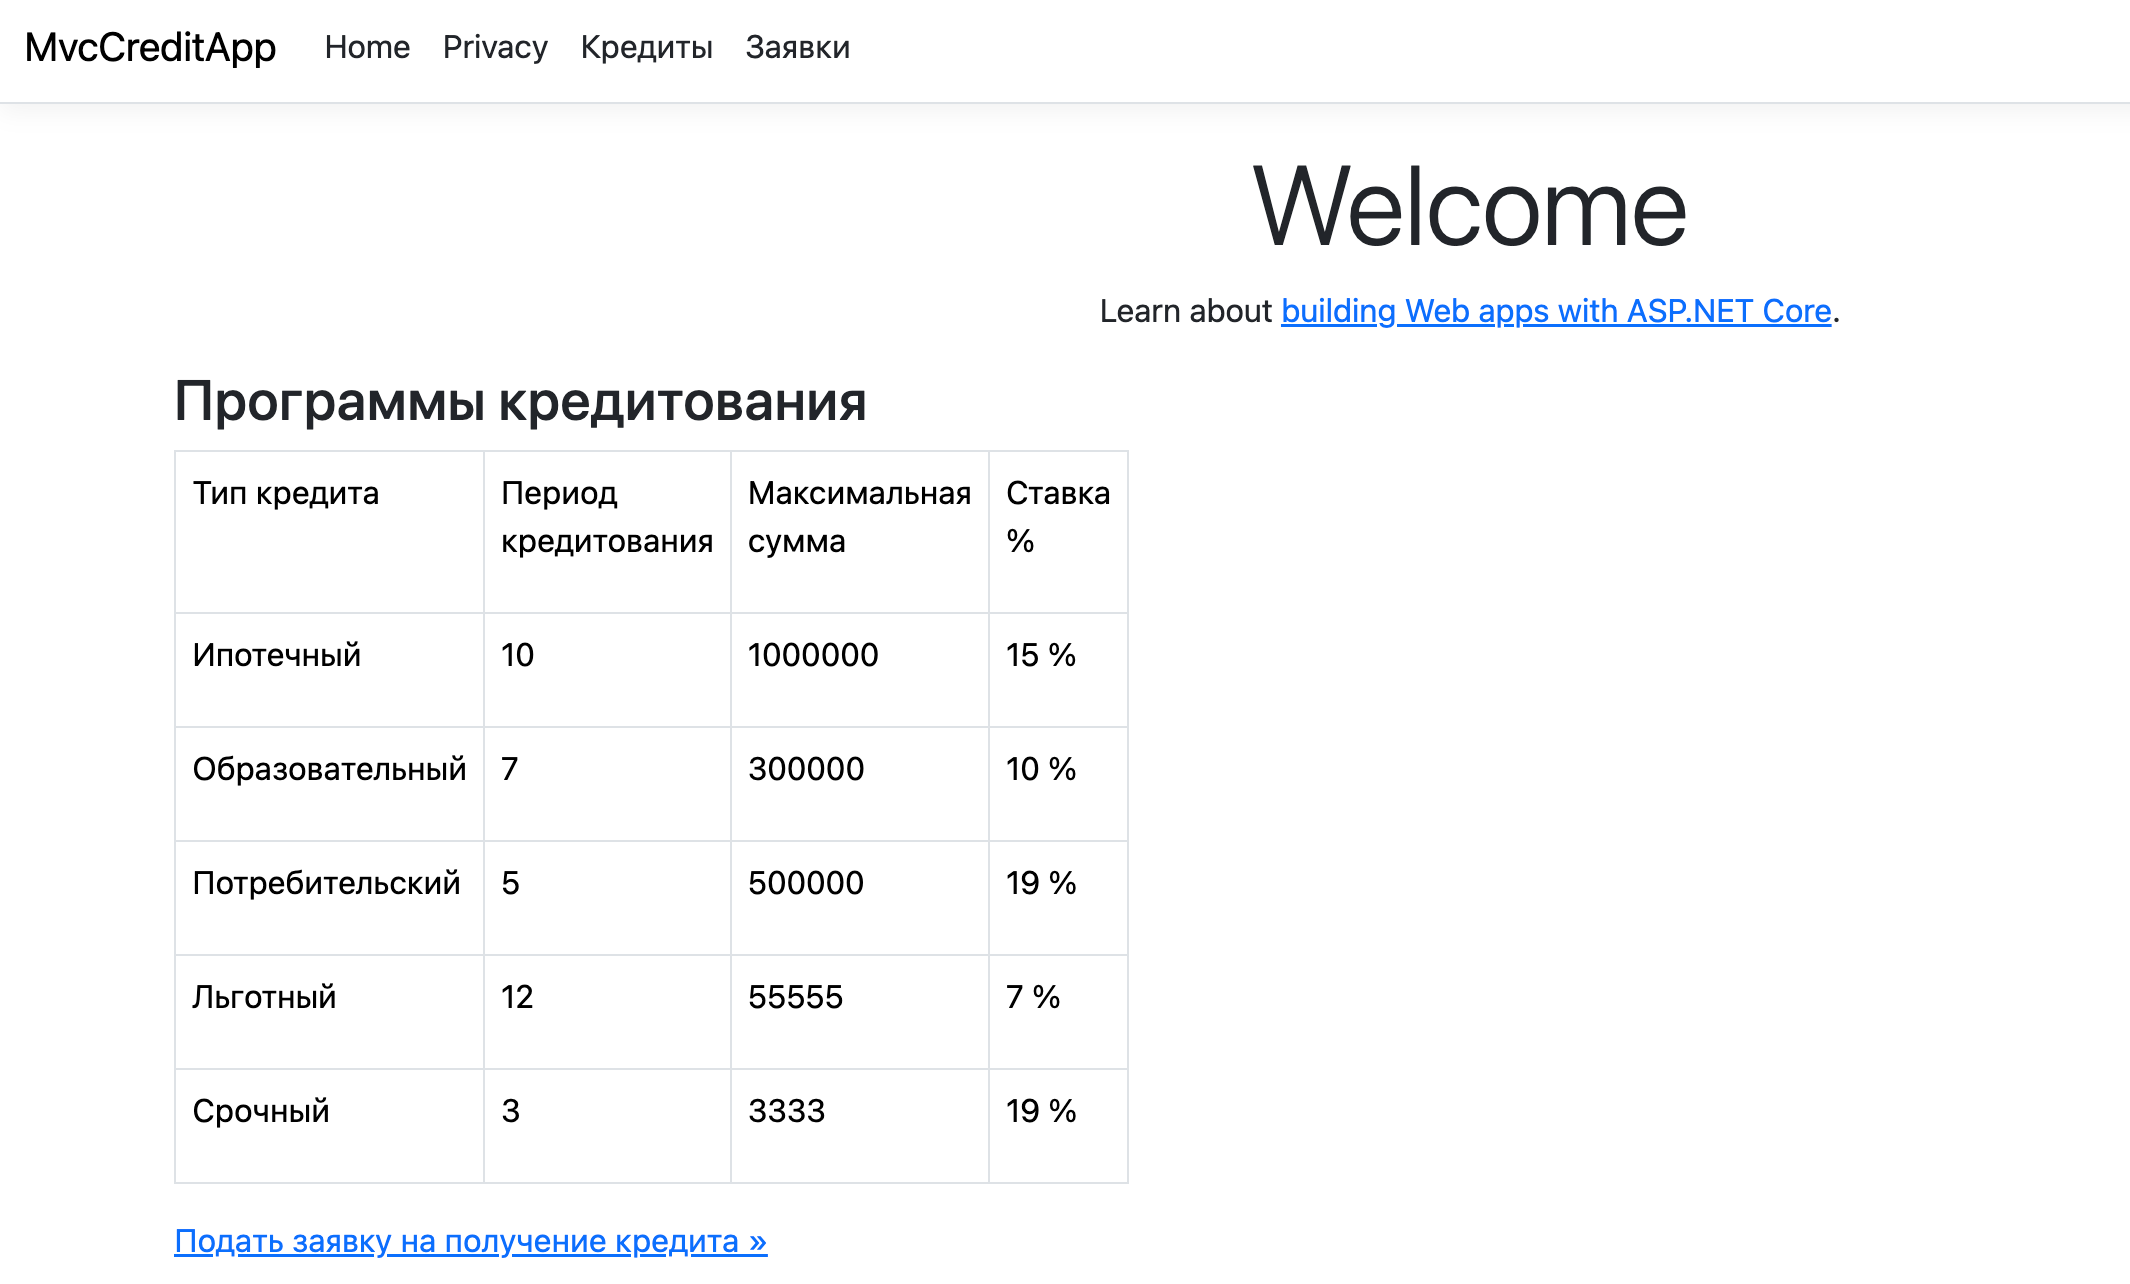
\includegraphics[width=0.8\textwidth]{../../скрины/SCR-20260328-pyve.png}
\caption{Главная страница с таблицей кредитов}
\end{figure}

На главной странице отображается таблица <<Программы кредитования>> с колонками: Тип кредита, Период, Максимальная сумма, Ставка. Внизу -- ссылка <<Подать заявку на получение кредита>>.

\section{ЛР 6. Scaffold-контроллеры и аннотации}

Через scaffolding сгенерированы \texttt{CreditsController} и \texttt{BidsController} с CRUD-действиями. Для каждого -- 5 представлений (Index, Details, Create, Edit, Delete), итого 10. К моделям добавлены аннотации \texttt{[DisplayName]} и \texttt{[Required]}. На Index кредитов установлен \texttt{[ResponseCache]}.

\begin{lstlisting}[caption={Метод CreateBid в HomeController},language={[Sharp]C}]
[HttpPost]
[ValidateAntiForgeryToken]
public async Task<IActionResult> CreateBid(Bid bid)
{
    if (ModelState.IsValid)
    {
        bid.bidDate = DateTime.Now;
        _context.Bids.Add(bid);
        await _context.SaveChangesAsync();
        return RedirectToAction("Index");
    }
    return View("Index");
}
\end{lstlisting}

\begin{figure}[H]
\centering
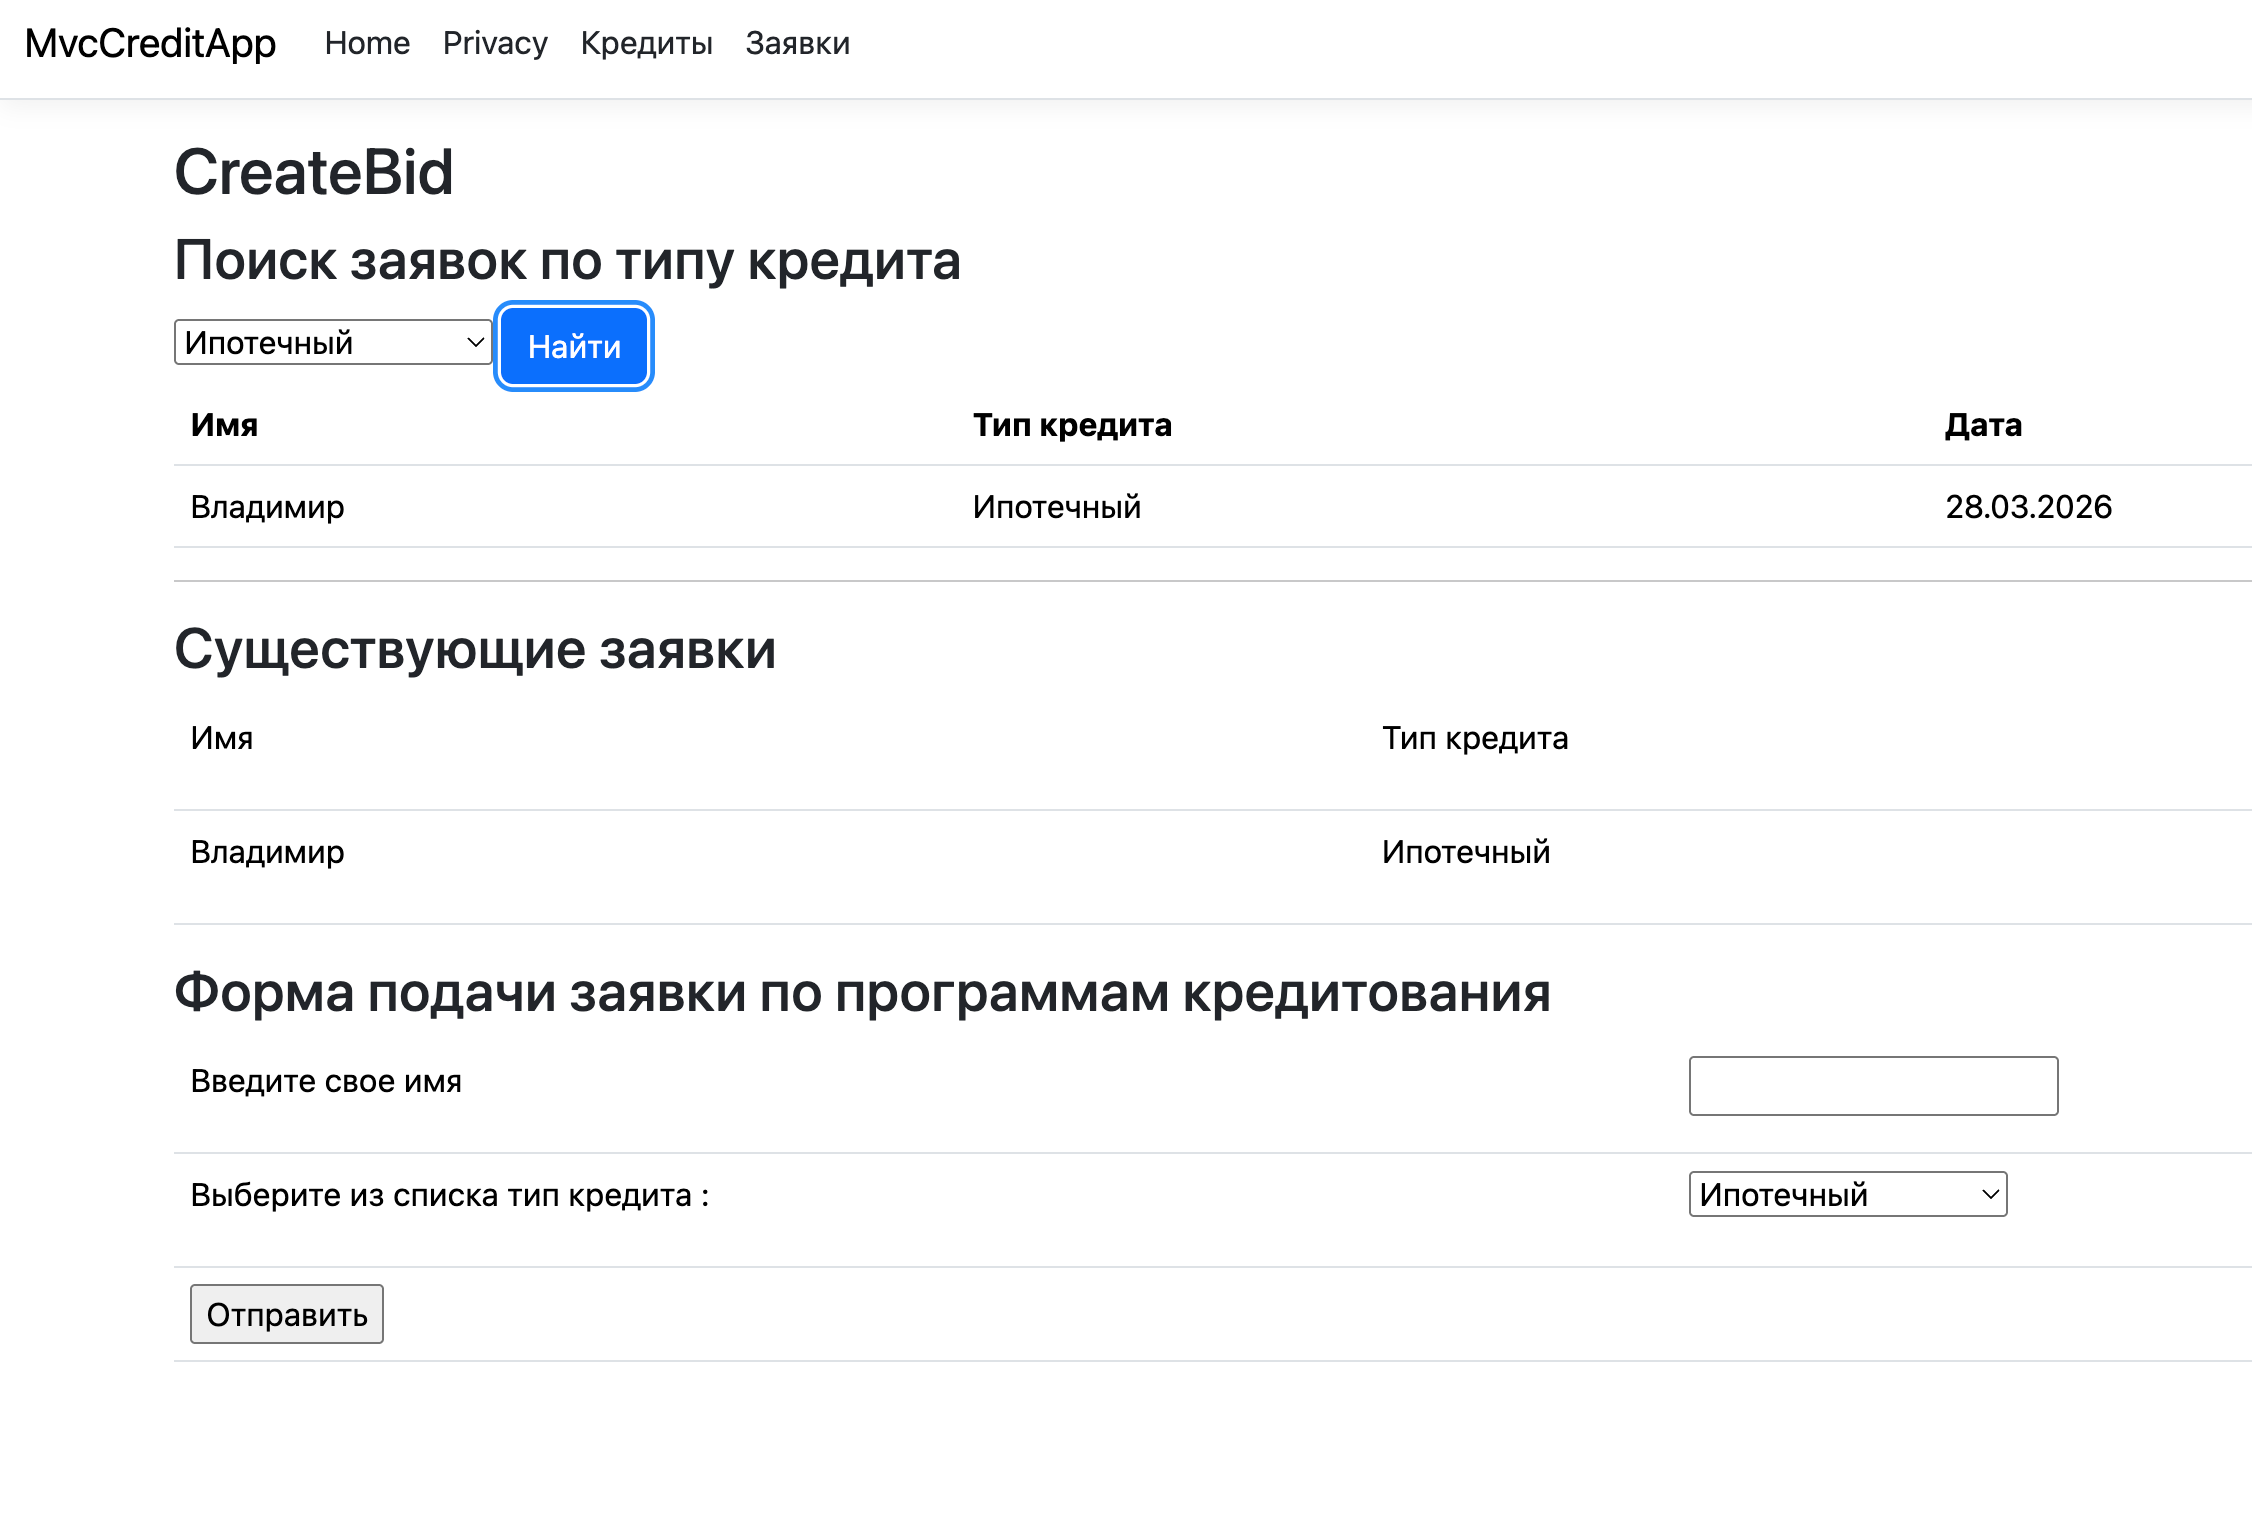
\includegraphics[width=0.8\textwidth]{../../скрины/SCR-20260328-pyxa.png}
\caption{Страница CreateBid с AJAX-поиском заявок}
\end{figure}

На странице \texttt{/Credits} (доступна только администратору) отображается список кредитов с возможностью создания, редактирования и удаления записей.

\section{ЛР 7. AJAX и частичные представления}

В \texttt{HomeController} добавлен метод \texttt{BidSearch} для поиска заявок по типу кредита. Результат возвращается через частичное представление \texttt{\_BidSearchPartial.cshtml}. Вместо \texttt{Ajax.BeginForm} используется \texttt{fetch()} API.

\begin{lstlisting}[caption={AJAX-поиск заявок},language={[Sharp]C}]
public IActionResult BidSearch(string creditHead)
{
    var bids = _context.Bids
        .Where(b => b.CreditHead == creditHead)
        .ToList();
    return PartialView("_BidSearchPartial", bids);
}
\end{lstlisting}

\begin{lstlisting}[caption={Скрипт fetch() на стороне клиента},language=html]
<script>
document.getElementById("searchBtn")
  .addEventListener("click", function() {
    var type = document.getElementById("creditType").value;
    fetch("/Home/BidSearch?creditHead=" + type)
      .then(r => r.text())
      .then(html => {
        document.getElementById("results").innerHTML = html;
      });
});
</script>
\end{lstlisting}

На странице \texttt{/Home/CreateBid} реализован поиск заявок: выбор типа кредита из выпадающего списка, кнопка <<Найти>>. Результат подгружается без перезагрузки страницы через AJAX.

\section{ЛР 8. Авторизация и аутентификация}

Настроена авторизация через ASP.NET Core Identity с ролями \texttt{admin} и \texttt{user}. При инициализации создаётся администратор (\texttt{admin@credit.com}).

\begin{lstlisting}[caption={Инициализация ролей в SeedData},language={[Sharp]C}]
public static async Task InitializeRoles(
    IServiceProvider serviceProvider)
{
    var roleManager = serviceProvider
        .GetRequiredService<RoleManager<IdentityRole>>();
    string[] roles = { "admin", "user" };
    foreach (var role in roles)
    {
        if (!await roleManager.RoleExistsAsync(role))
            await roleManager.CreateAsync(
                new IdentityRole(role));
    }
}
\end{lstlisting}

На метод \texttt{CreateBid} установлен атрибут \texttt{[Authorize]}, требующий авторизации для подачи заявки. CRUD-операции с кредитами и удаление заявок доступны только администраторам через \texttt{[Authorize(Roles = "admin")]}.

\begin{figure}[H]
\centering
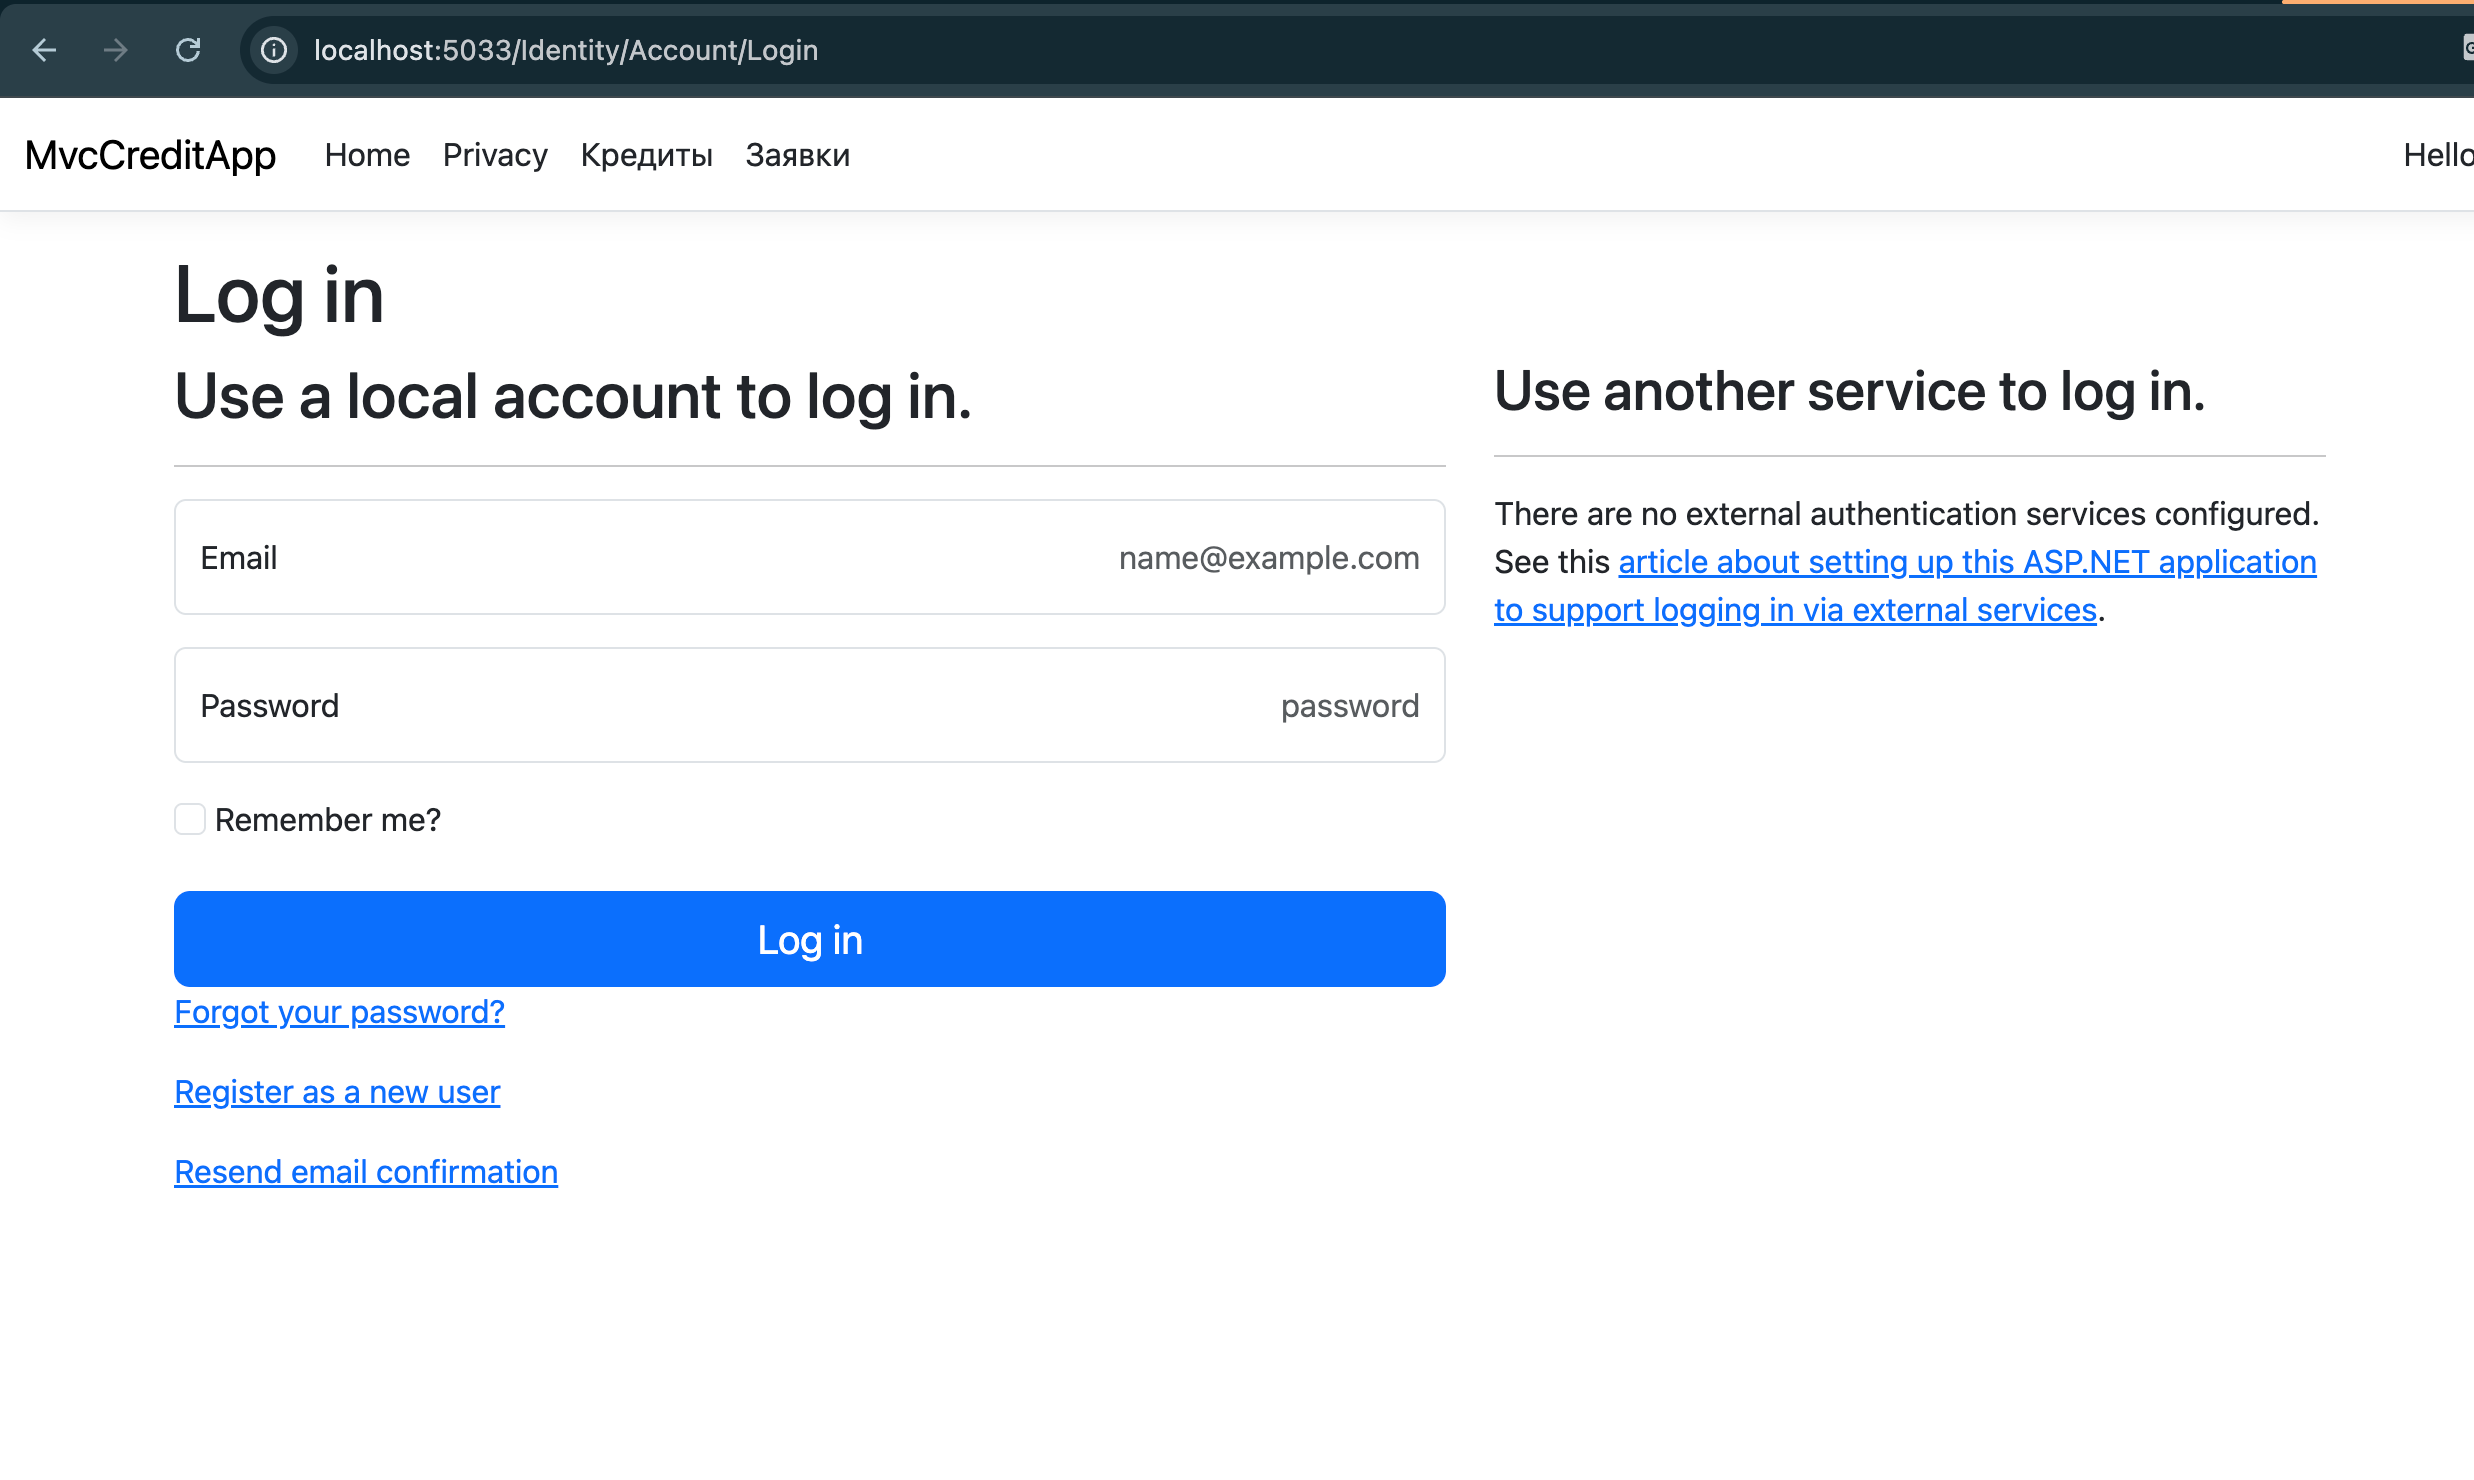
\includegraphics[width=0.8\textwidth]{../../скрины/SCR-20260328-pyyk.png}
\caption{Страница входа Identity}
\end{figure}

Страница входа \texttt{/Identity/Account/Login} содержит форму с полями Email и Password, а также ссылки на регистрацию и восстановление пароля.

\section{Заключение}

В ходе лабораторных работ 5--8 разработано MVC-приложение для управления кредитными продуктами. Реализованы модель данных с Entity Framework Core, CRUD-контроллеры через scaffolding, AJAX-поиск с частичными представлениями и система авторизации с разделением ролей. Приложение работает на SQLite и поддерживает регистрацию, вход и разграничение доступа.

\end{document}
